\chapter{不相交路径问题}


不相交路径(Disjoint Path) 问题可以看作是最短路径问题的一个扩展,是网络故障恢复路径保护方法的主要技术。不相交路径是计算出几条不共享任何公共点/边的路径。提供不相交路径将提高网络连接的可靠性和网络流量,并相应地提高网络的可生存性。网络可生存性被定义为在网络组件(例如,节点/链路)发生故障时提供持续服务的能力\cite{zhou2000survivability}。 不相交路径对问题是不相交路径问题的另一个变体。

不相交路径具有广泛的应用领域。例如,对于通信网络中的业务具有多条不相交的路径将提高其传输可靠性。通过在多个不相交路径上并发发送流量,路径的失效不会影响其他路径的性能,并且流量仍将到达其目的地。在交通网络中,预先计算出的不相交路径数将使卡车司机能够按照不同的路径改变路线,而不是总是坚持最短的路径。

%maritime network freights

本章的其余部分按以下方式组织。在\textbf{不相交路径}部分,给出了不相交路径的形式化定义,讨论不相交路径问题的附加条件限制及其相应的时间复杂性,描述了几种有代表性的不相交路径算法。在\textbf{基于可靠性的不相交路径}部分,我们将介绍路径可靠性的概念及其与不相交路径的关系。在\textbf{最大不相交路径}部分将阐述不相交路径可能部分重叠的情况下而不是完全不相交。在域不相交路径章节,我们继续在多域网络中寻找域不相交路径。因为多个链接(或多个节点)可能在共享风险下同时失效,在\textbf{共享风险链路组不相交路径}部分介绍共享风险链接组SRLG的概念。确保不相交的路径不会同时失效由于单个链接(或节点)失败。风险也可能影响基于地区的网络,因此\textbf{地区不相交路径}部分讨论了几种基于地区的风险模型。与不相交路径问题对应的不相交路径对问题将在\textbf{不相交路径对}部分中讨论,将讨论不同情况下的复杂性。最后,我们在最后一节对本章进行了简要的总结。

\section{预备知识}
%\subsection{图论}
网络在我们的日常生活中非常普遍。我们的身体是由突触连接的神经元网络组成的。我们的运输网络使我们能够轻松地往返于不同的地方。互联网是我们巨大的信息门户也是世界内的计算机网络。电网提供电力,而如果没有电力那我们现在社会都可能会停止运作。我们的社交网络让我们和朋友与家人联系。由于网络的重要性,网络特性的多样性已经得到了广泛的研究,尤其是在图论领域。

在图论中,网络被看作是一种通过节点互相链接的。节点表示网络的关节点,例如,通信网络中的路由器,海运网络或交通网络中的城市。链路表示将关键点连接在一起的连接器,例如,通信网络中的电缆,海运中的贸易路线,运输网络中的网络或公路。

图论中研究最多的课题之一是最短路径问题,即在网络中的两个节点,使得路径上链路权重之和最小化。传统的最短路径算法是Dijkstra算法\cite{dijkstra1959note}以及Bellman-Ford 算法\cite{toth2002vehicle,ford2015flows}。 使用最短路径在一个通信网络的两个路由器间信号可以在最小延迟之间交换,货物可以在海运网络中两个港口之间的以燃油成本最低的代价发送,而且在运输网络中我们可以更快地往返于城市之间。

网络通常表示为图$G(\mathbb{V},\mathbb{E})$,其中$\mathbb{V}$是$|\mathbb{V}|$ 个节点的集合(例如,节点表示路由)和$\mathbb{E}$是$|\mathbb{E}|$ 条链路的集合(例如,链路代表光纤线路或无线电信道)。链接可能带有延迟、长度或成本等属性。对于每条链路$e_i$,$w_{e_i}$表示链路的权重。路径$P$的权重表示为路径$P$中每条链路的权重之和$w_P=\sum\limits_{e_i\in \mathbb{P}}w_{e_i}$。
\section{不相交路径}
不相交路径问题被定义成如下:

\begin{definition}[不相交路径问题]
给定$|\mathbb{V}|$个节点集$\mathbb{V}$和 $|\mathbb{E}|$条加权链路集 $\mathbb{E}$ 组成的有向网络 $G(\mathbb{V},\mathbb{E})$,两个特殊节点$s,d\in\mathbb{V}$。 给定一个整数$k>0$,求$s$到$d$的$k$ 条路径$P_1,P_2,\ldots,P_k$,使路径间不共享任何公共链路(或节点)。
\end{definition}

对不相交的路径添加附属目标条件,例如:
\begin{itemize}
  \item 最小-最大(Min-Max)不相交路径问题--所有链路权重之和最大的路径最小化。
  \item 最小-最小(Min-Min)不相交路径问题--所有链路权重之和最小的路径最小化。
  \item 有界(Bounded)不相交路径问题--每条路径的所有链路权重之和应小于给定权值$\bigtriangleup$.
  \item 最小和(Min-Sum)不相交路径问题--$k$条路径的所有链路权重之和的总和最小化。
\end{itemize}
算法\ref{alg:IterativeDP}给出了求解不相交路径问题的一种简单的启发式算法,称为迭代DP算法。迭代DP算法基于$k$个连续最短路径的计算。

\begin{algorithm}[htbp]
{
{
\renewcommand\baselinestretch{1.5}\selectfont %控制行距
\caption{迭代DP算法}
\label{alg:IterativeDP}
\begin{algorithmic}[1]
    \FOR{$i\leftarrow\ 1\ to\ M$}
        \STATE{寻找从节点$s$到节点$d$的最短路径$P_i$}
        \STATE{从$G$中删除$P_i$的中间节点链路}
    \ENDFOR
\end{algorithmic}
}
\par}
\end{algorithm}

Bhandari\cite{bhandari1997optimal}提出了一种不受到陷阱拓扑影响的Min-Sum不相交路径算法。虽然有一种称为Suurballe算法\cite{suurballe1974disjoint}也可以绕过陷阱拓扑问题,但我们关注Bhandari 算法,因为它更简单。算法\ref{alg:Bhandari}给出了Bhandari算法的伪码,我们演示了使用Bhandari算法在图\ref{fig:bhandariP1}所示的网络查找$k=3$ 条链路不相交的路径(从节点1到节点5)。从节点1到节点5的第一条初步最短路径是$P_1=1-2-3-4-5$(权重4)。$P_1$的组成链路反转其链路权重取负如图\ref{fig:bhandariLinkReversal}所示。然后,计算的另一条初步最短路径$P_2=1-4-3-5$(权重8),如图\ref{fig:bhandariP2}所示。为了得到两条链接不相交的路径$P_1$和$P_2$,不包括重叠链路,在计算另一条初始路径$P_3=1-3-2-6$(权重9) 之前,第3-5行再次重复,如图\ref{fig:bhandariP3} 所示。再次,将重叠链路排除在外,以获得最后三条链路不相交的路径,如图\ref{fig:bhandariP1P2P3}所示。

\begin{figure}[htbp]
  \centering
  \subfigure[$P_1$]{
            \label{fig:bhandariP1}
            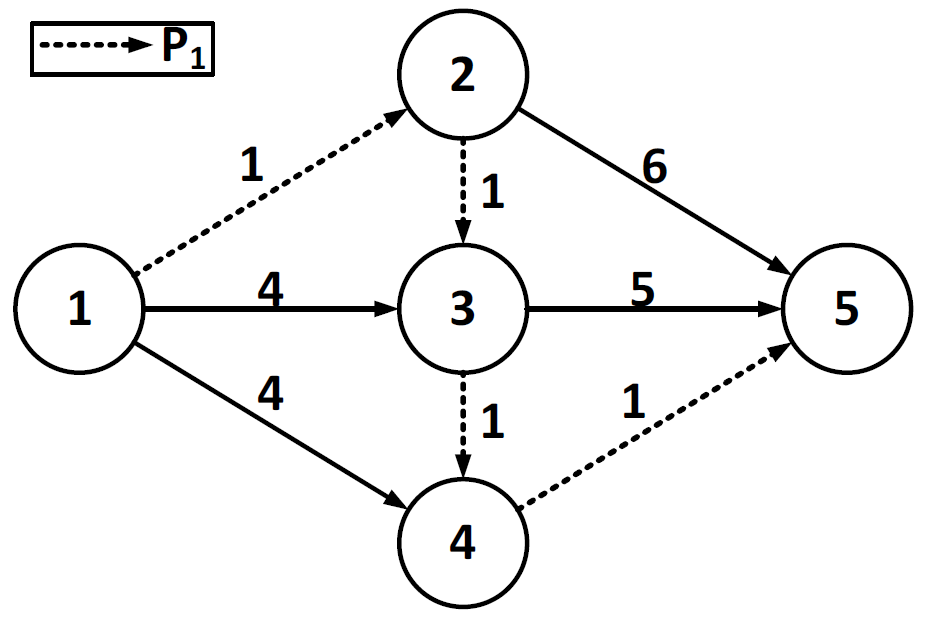
\includegraphics[width=0.4\textwidth]{figures/bhandariP1}}
  \subfigure[链路反转]{
            \label{fig:bhandariLinkReversal}
            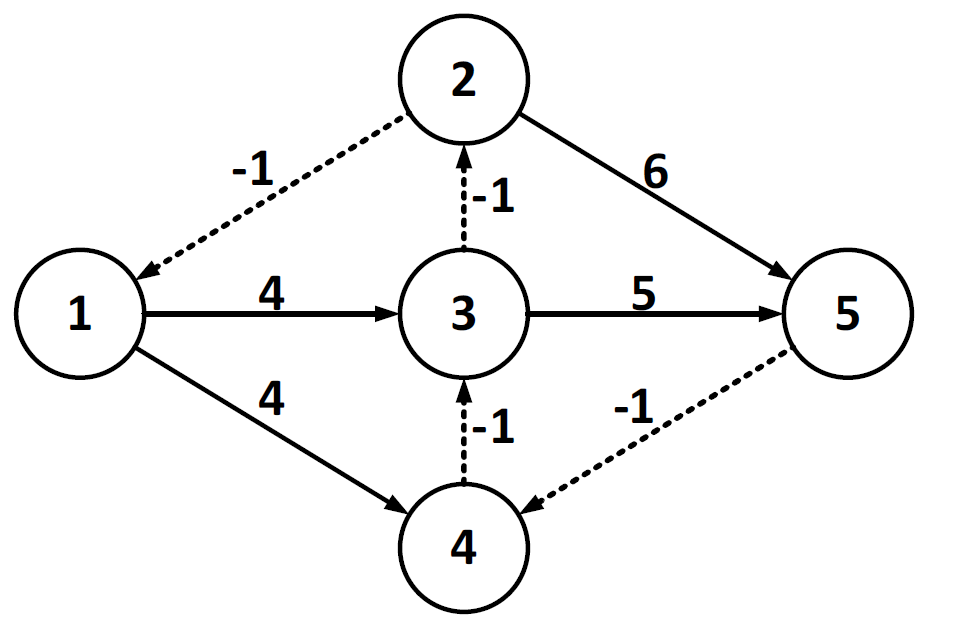
\includegraphics[width=0.4\textwidth]{figures/bhandariLinkReversal}}
  \subfigure[$P_2$]{
            \label{fig:bhandariP2}
            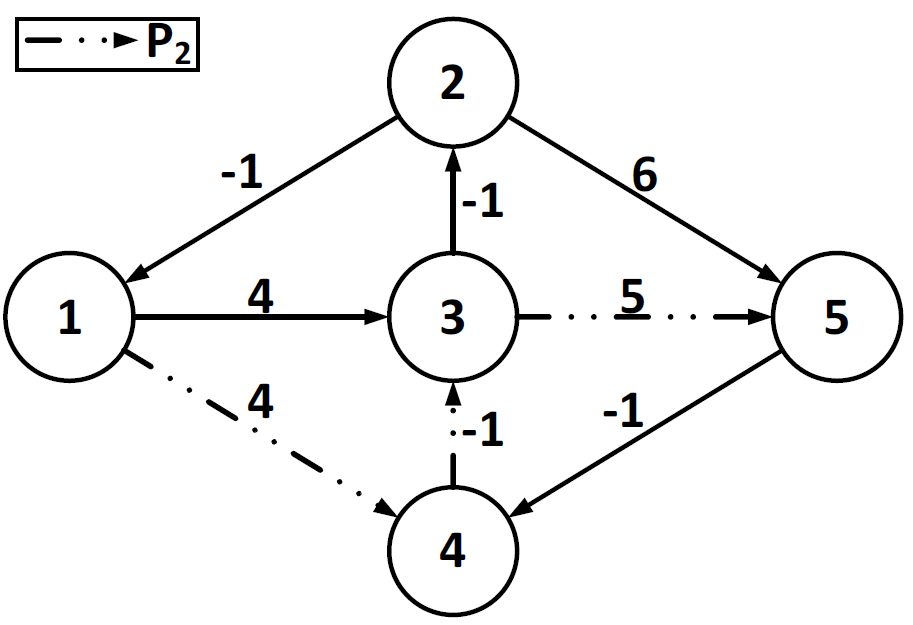
\includegraphics[width=0.4\textwidth]{figures/bhandariP2}}
  \subfigure[$P_3$]{
            \label{fig:bhandariP3}
            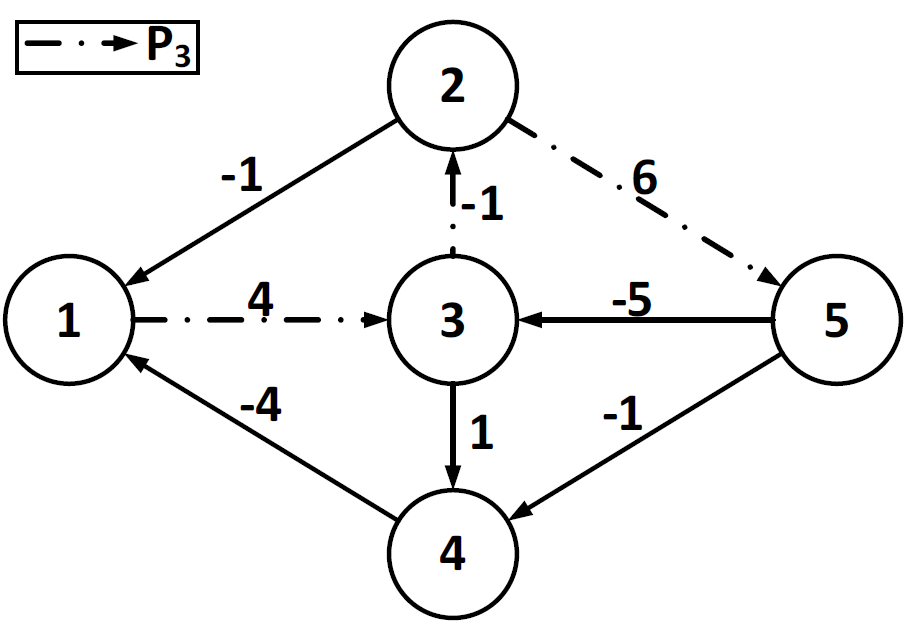
\includegraphics[width=0.4\textwidth]{figures/bhandariP3}}
  \subfigure[非重叠 $P_1,P_2$ 和 $P_3$]{
            \label{fig:bhandariP1P2P3}
            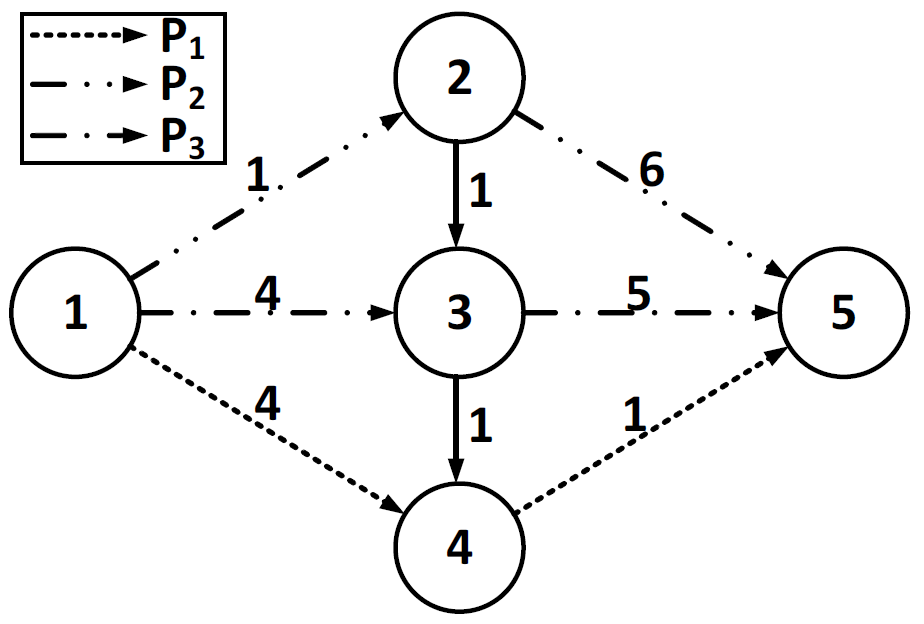
\includegraphics[width=0.4\textwidth]{figures/bhandariP1P2P3}}
  \caption{Bhandari算法实例}\label{fig:BhandariAlg}
\vspace{\baselineskip}
\end{figure}

\begin{algorithm}[!h]
{
{
\renewcommand\baselinestretch{1.5}\selectfont %控制行距
\caption{Bhandari$(G,s,t,k)$}
\label{alg:Bhandari}
\begin{algorithmic}[1]
    \STATE{寻找从节点$s$到节点$d$的最短路径$P_1$}
    \FOR{$i\leftarrow\ 2\ to\ M$}
        \STATE{对于节点不相交的路径,拆分所有$P_x$的中间节点,其中$x<i$}
        \STATE{用反向边替换在原图中所有$P_x(x<i)$路径的每条链路}
        \STATE{寻找从节点$s$到节点$d$的最短路径$P_i$}
        \STATE{删除所有重叠链接,以获得不相交的路径$P_x$,其中$x\leq i$}
    \ENDFOR
\end{algorithmic}
}
\par}
\end{algorithm}

%\begin{algorithm}[!h]
%{
%{
%\renewcommand\baselinestretch{1.5}\selectfont %控制行距
%\caption{ Scheduling Algorithm }
%\label{alg:schedule}
%\begin{algorithmic}[1]
%\REQUIRE ~\\
%A DFG $G=<V,E>$;\\
%An allocation $A(G)$ for $G$.
%\ENSURE ~\\
%A schedule.
%    \STATE{.......................}
%    \FOR{$i\leftarrow\ 1\ to\ M$}
%        \STATE{.......................}
%    \ENDFOR
%    \STATE{.......................}
%    \STATE{.......................}
%    \STATE{.......................}
%    \STATE{.......................}
%    \STATE{.......................}
%    \FOR{$k\leftarrow\ 1\ to\ |V|$}
%        \STATE{.......................}
%        \STATE{.......................}
%        \STATE{.......................}
%        \STATE{.......................}
%    \IF{$LT_k==j$}
%        \IF{there is no idle core in cluster $cl_{loc}$}
%            \STATE{.......................}
%            \STATE{.......................}
%            \STATE{.......................}
%            \STATE{.......................}
%            \STATE{.......................}
%            \STATE{.......................}
%        \ELSE
%            \STATE{.......................}
%            \STATE{.......................}
%            \STATE{.......................}
%            \STATE{.......................}
%            \STATE{.......................}
%            \STATE{.......................}
%        \ENDIF
%    \ENDIF
%    \ENDFOR
%
%
%\end{algorithmic}
%}
%\par}
%\end{algorithm}
\section{可靠性不相交路径}
路径可靠度是指路径在未来随机时间内处于运行状态的概率\cite{clouqueur2002availability}。 路径$P$的可靠度($A$) 可以通过乘以其所有组成链路的可靠度来计算:
\begin{equation}
A=\prod_{y\in P}a_y
\end{equation}

其中$a_y$是链路y的可靠度,它依赖于链路的平均故障间隔时间(MTBF)和平均修复时间(MTTR)。
\begin{equation}
a=\frac{MTBF}{MTBF+MTTR}
\end{equation}
\begin{equation}
MTBF=\frac{total\ operating\ time}{number\ of\ failures}=\frac{1}{failure\ rate}
\end{equation}
\begin{equation}
MTTR=failure\ localization\ time+failure\ repair\ time
\end{equation}
k条不相交路径的总可靠度可以计算为:
\begin{equation}
A_t=1-\prod_k(1-A_k)
\end{equation}
可靠性不相交路径问题被定义成如下:

\begin{definition}[可靠性不相交路径]
给定$|\mathbb{V}|$个节点集$\mathbb{V}$和 $|\mathbb{E}|$条加权链路集 $\mathbb{E}$ 组成的有向网络 $G(\mathbb{V},\mathbb{E})$,两个特殊节点$s,d\in\mathbb{V}$,给定一个整数$k>0$ 和小数$\delta$,每条链路的权重即为每条链路的可靠度,求$s$ 到$d$ 的$k$ 条路径$P_1,P_2,\ldots,P_k$,使路径间不共享任何公共链接(或节点)并且$k$ 条路径总的可靠度$A_t$ 至少为$\delta$。
\end{definition}
\section{最大不相交路径}
最大不相交路径问题被定义成如下:

\begin{definition}[最大不相交路径问题]
给定$|\mathbb{V}|$个节点集$\mathbb{V}$和 $|\mathbb{E}|$条加权链路集 $\mathbb{E}$ 组成的有向网络 $G(\mathbb{V},\mathbb{E})$,两个特殊节点$s,d\in\mathbb{V}$,给定一个整数$k>0$,求$s$到$d$的$k$ 条路径$P_1,P_2,\ldots,P_k$,使路径间共享最少的公共链接(或节点)。
\end{definition}
如果不存在完全不相交的路径,则最大不相交路径是有用的。如果两个路径所共有的(节点)链路的数目最小,则一对路径是最大不相交的。如图\ref{fig:MaximallyDisjointPaths}所示,因为不存在完全不相交的路径对,从节点1到节点4的路径$P_1$和$P_2$都使用链路(3,4)。然而,如果共享节点或链路失效,最大不相交路径仍然容易出现同步路径失效。例如,如果链接(3,4)失效,则$P_1$ 和$P_2$路径都将失效。
\begin{figure}[htbp]
  \centering
  % Requires \usepackage{graphicx}
  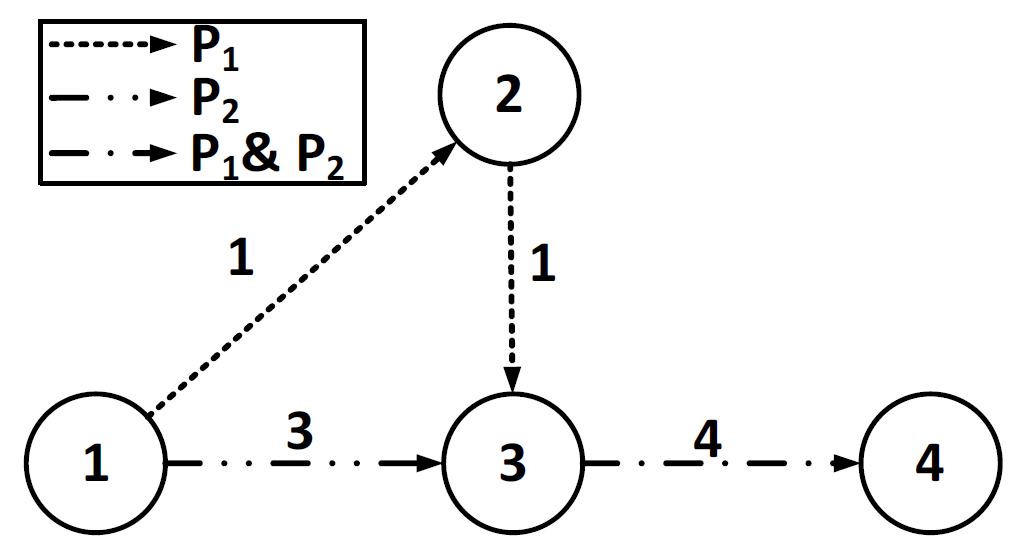
\includegraphics[width=4.0in]{figures/MaximallyDisjointPaths}
  \caption{最大不相交路径的实例}
  \label{fig:MaximallyDisjointPaths}
\end{figure}

\section{域不相交路径}
域不相交路径问题被定义成如下:

\begin{definition}[域不相交路径问题]
给定$|\mathbb{V}|$个节点集$\mathbb{V}$,$|\mathbb{E}|$条加权链路集 $\mathbb{E}$,$|\mathbb{D}|$个域集$\mathbb{D}$,$|\mathbb{L}|$条域内加权链路集 $\mathbb{L}$ 组成的有向网络 $G(\mathbb{V},\mathbb{E},\mathbb{D},\mathbb{L})$,两个特殊节点$s,d\in\mathbb{V}$。每个域$d\in\mathbb{D}$由一组点集$\mathbb{V}_d\subseteq \mathbb{V}$和一组由点集$\mathbb{V}_d$ 构成的链路集$\mathbb{E}_d\subseteq \mathbb{E}$构成。给定一个整数$k>0$,求$s$ 到$d$ 的$k$ 条路径$P_1,P_2,\ldots,P_k$,使路径间不共享任何公共域。
\end{definition}

域是由一组节点和链路组成。图\ref{fig:MultiDomainNetwork}所示了一个具有四个域的网络,这些域通过域间链路相互连接。域可以表示光网络中的行政区域、交通网络中城市的一个省等。

\begin{figure}[htbp]
  \centering
  % Requires \usepackage{graphicx}
  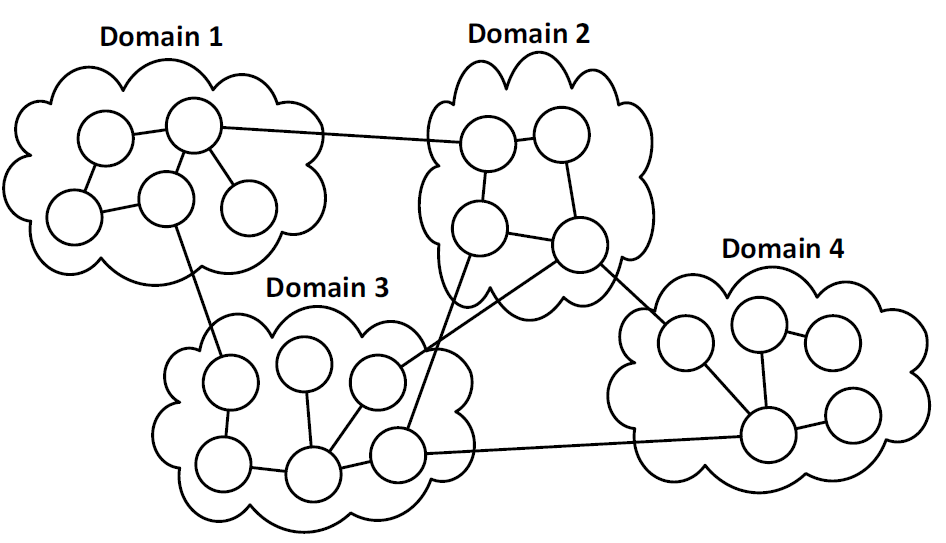
\includegraphics[width=4.0in]{figures/MultiDomainNetwork}
  \caption{多域网络实例}
  \label{fig:MultiDomainNetwork}
\end{figure}
\section{地区不相交路径}
地区不相交路径问题被定义成如下:

\begin{definition}[地区不相交路径问题]
给定$|\mathbb{V}|$个节点集$\mathbb{V}$和 $|\mathbb{E}|$条加权链路集 $\mathbb{E}$ 组成的有向网络 $G(\mathbb{V},\mathbb{E})$,并且这些点和边被嵌入到二维平面中,两个特殊节点$s,d\in\mathbb{V}$和一个直径$D>0$。 给定一个整数$k>0$,求$s$ 到$d$ 的$k$ 条路径$P_1,P_2,\ldots,P_k$,使路径间不会受到直径$D$ 的单一地区失效的影响(除了在点$s,d$ 中的失效)。
\end{definition}

例如,如图\ref{fig:RegionDisjointPath}所示的网络链路的权重代表其相邻节点之间公里距离。考虑当$D=15 km$时从节点1到节点6找一对地区不相交路径的问题。由于链路(2,4)和(3,5)之间的距离小于D,路径$P_1$和$P_1$不是该问题的可行解决方案。


\begin{figure}[htbp]
  \centering
  % Requires \usepackage{graphicx}
  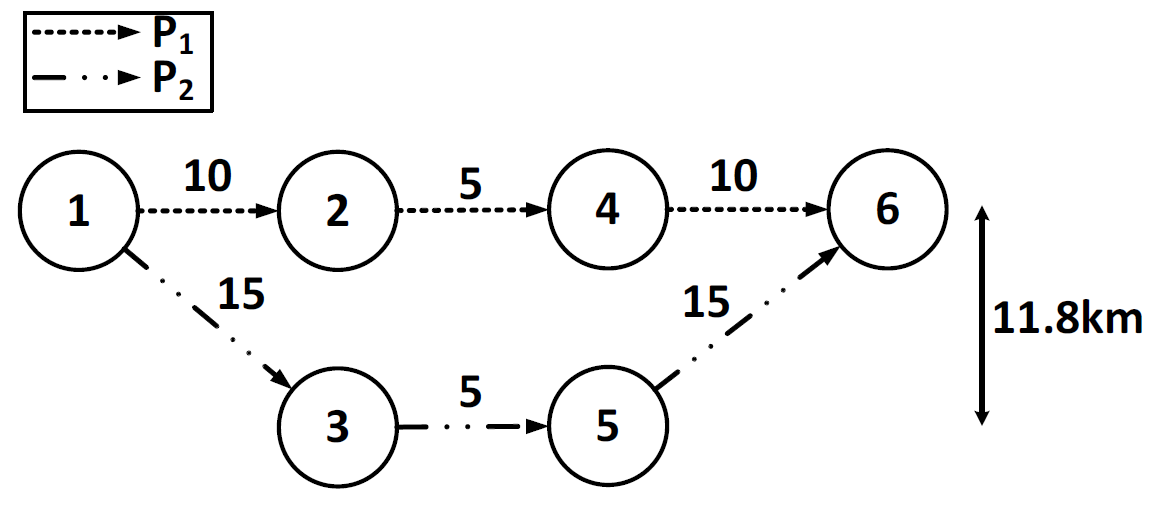
\includegraphics[width=4.5in]{figures/RegionDisjointPath}
  \caption{地区不相交路径的实例}
  \label{fig:RegionDisjointPath}
\end{figure}
\section{不相交路径对}
不相交路径对问题被定义成如下:

\begin{definition}[不相交路径对]
给定$|\mathbb{V}|$个节点集$\mathbb{V}$和 $|\mathbb{E}|$条加权链路集 $\mathbb{E}$ 组成的有向网络 $G(\mathbb{V},\mathbb{E})$,$k$对特殊节点对$s_k,d_k\in\mathbb{V}$。给定一个整数$k>0$,求$k$ 条路径$P_1,P_2,\ldots,P_k$ 分别从其对应的源节点$s_k$到其对应的目的节点$d_k$,使路径间不共享任何公共链接(或节点)。
\end{definition}
例如,图\ref{fig:DisjointPathPairs}所示的不相交路径对$P_1,P_2,P_3$和$P_4$都是不相交的。
\begin{figure}[htbp]
  \centering
  % Requires \usepackage{graphicx}
  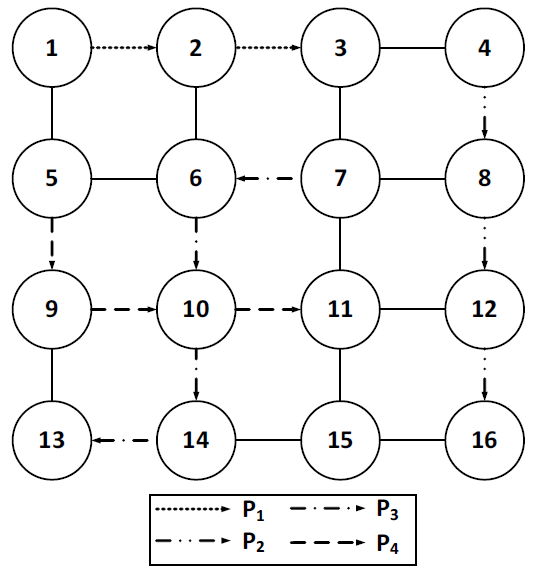
\includegraphics[width=3.0in]{figures/DisjointPathPairs}
  \caption{不相交路径对实例}
  \label{fig:DisjointPathPairs}
\end{figure}
\section{共享风险链路组不相交路径}






共享风险链路组不相交路径问题定义如下:

\begin{definition}[共享风险链路组不相交路径问题]
给定$|\mathbb{V}|$个节点集$\mathbb{V}$和 $|\mathbb{E}|$条加权链路集 $\mathbb{E}$ 组成的有向网络 $G(\mathbb{V},\mathbb{E})$和$|\mathbb{R}|$ 个风险组$\mathbb{R}$,两个特殊节点$s,d\in\mathbb{V}$。 任何链路$(u,v)\in\mathbb{E}$,给定一个整数$k>0$,求$s$ 到$d$ 的$k$ 条路径$P_1,P_2,\ldots,P_k$,使路径间不共享任何公共风险组。
\end{definition}
风险组里的资源可以是节点而不一定是链路,这就引申出共享风险节点组不相交路径问题。共享风险节点组不相交路径可以通过节点转移方法成共享风险链路组不相交路径问题。

%\subsection{概率共享风险链路组}
%当前的链路故障恢复算法大多是针对独立故障的,而事实上有时候链路故障并不是完全独立的,比如当底层光纤链路故障时,由其承载的多条逻辑链路可能会同时失效,即链路故障之间存在概率关联。当SRLG 中的一条链路失效时,该组中其它链路以100\%的概率出现失效。但实际上关联故障并非100\%绝对关联,拥有关联故障的两条链路中的一条链路发生故障时,另一条链路只是以某一概率发生故障。为此,我们给出了概率共享风险链路组概念,在传统的SRLG 模型中加入故障关联概率来表示拥有一定概率关联的故障模型。
%\begin{definition}[概率共享风险链路组(Probabilistically Shared Risk Link Group, PSRLG)]
%设$\mathbb{R}$为SRLG集合,当任意事件$r\in\mathbb{R}$发生时,故障发生概率不为0的链路集合构成事件r的PSRLG,如式\ref{equ:PSRLG}所示。
%\begin{equation}\label{equ:PSRLG}
%  r_{PSRLG}=\{e_{i,j}\in \mathbb{E}:p_r(i,j)\neq 0\}
%\end{equation}
%其中$p_r(i,j)$为SRLG事件r发生时链路$e_{i,j}$发生故障
%的概率。
%\end{definition}
%链路$e_{i,j}$与链路$e_{u,v}$之间存在故障关联是指当某事件r发生时,$p_r(i,j)\neq 0$且$p_r(u,v)\neq 0$。而传统的SRLG 模型中,链路$e_{i,j}$与链路$e_{u,v}$之间存在故障关联是指事件r发生时,$p_r(i,j)=1$ 且$p_r(u,v)=1$,显然传统的SRLG 模型只是概率关联模型的一个特例。利用概率关联故障模型可以更加真实地刻画关联故障的特点。用$p_r$表示事件r发生概率,链路$e_{i,j}$和$e_{u,v}$存在故障关联时,各自发生故障的概率分别用$p_{u,v}$和$p_{i,j}$
%表示。
%\begin{equation}\label{equ:PSRLpuv}
%  p_{u,v}=p_r*p_r(u,v)
%\end{equation}
%\begin{equation}\label{equ:PSRLpij}
%  p_{i,j}=p_r*p_r(i,j)
%\end{equation}
%根据式\ref{equ:PSRLpuv}和式\ref{equ:PSRLpij},只有当$p_r\neq 0$时, $p_{u,v}$与$p_{i,j}$不为0,即链路$e_{i,j}$与$e_{u,v}$当存在故障关联时同时受到事件$r$的影响各自发生故障的概率。利用概率关联故障模型我们可以非常方便地得到存在关联故障链路发生故障的概率。

%\section{共享风险节点组不相交路径}
\section{小结}
如表\ref{tab:disjointPath}概述了所考虑的不相交路径问题的变体。每个问题都根据其约束条件、实际应用和时间复杂度进行分类。

\begin{table}[htb]
\caption{不相交路径算法比较}\label{tab:disjointPath}
\vspace{0.5em}\centering\wuhao
\begin{tabularx}{46em}{|*{4}{>{\centering\arraybackslash}X|}}
\toprule[1.5pt]
问题   & 约束条件   & 实际应用 & 时间复杂度  \\
\midrule[1pt]
不相交路径 & 路径不共享公用链路或节点 & 为运输网络中的卡车司机提供不同的候选路径 & 多项式可解(例如Bhandari算法\cite{bhandari1997optimal})\\
\hline
可靠性不相交路径 & 路径不共享公共链接或节点,具有可靠性约束 & 提高电信网络中业务的连接可靠性 & 多项式可解(例如Bhandari算法\cite{bhandari1997optimal})\\
\hline
最大不相交路径 & 路径共享最小的公共链路或节点 & 在两个地点安全地转移一个非常重要的人 & NP-hard和很难有近似算法其因子为$2^{log^{1-\epsilon}N}(\epsilon>0)$。 当k=2 时,这个问题是多项式可解(例如MADSWIP算法\cite{taft1999quality})\\
\hline
域不相交路径 & 路径不共享公共域 & 提高跨多个光网络域的业务传输可靠性。 & NP-hard\cite{gao2013domain}\\
\hline
地区不相交路径 & 路径不能受到直径D的单一地区失效的影响(除了包括源或目标节点失效) & 确保地区灾难不会同时影响不同不相交的道路 & NP-hard和很难有近似算法\cite{trajanovski2015finding},除非所有成对的网络节点距离大于$D$\\
\hline
不相交路径对 & 路径不共享公共链路或节点(路径间可能有不同的源节点和目标节点)。 & 在芯片上互连指定的通道,没有任何不同引脚的电线相互接触 & 当$k\geq2$在一般有向网络中为NP-hard\cite{fortune1980directed},但在无向网络\cite{robertson1995graph}、 有向平面网络\cite{schrijver1994finding}和有向无圈网络中\cite{fortune1980directed} 是多项式可解的 \\
\hline
风险共享链路组不相交路径 & 路径不共享共同的风险组 & 确保不同的不相交路径不使用属于光网络中同一管道的链路。 & NP-hard\cite{hu2003diverse} 和难以近似\cite{coudert2007shared},除非所有SRLG遵循星型性质且所有SRLG的数目为常数\cite{bermond2013srlg},或当所有SRLG遵循星性且最大节点度最多为4\cite{bermond2013srlg} 时,或者当所有SRLG遵循星型性质且网络是有向无圈图\cite{bermond2013srlg}时,或在特定跨度共享拓扑\cite{bhandari1994optimal}中\\
\bottomrule[1.5pt]
\end{tabularx}
\vspace{\baselineskip}
\end{table}
